\documentclass[12pt]{article}
\usepackage
[
a4paper,
left=1.5cm,
right=2cm,
top=1.5cm,
bottom=1.5cm,
]
{geometry}
%\usepackage{ucs}
 \usepackage[utf8x]{inputenc}
\usepackage{multirow}
%\usepackage[utf8x]{inputenc}
\usepackage{mathtools}
\usepackage{listings}
\usepackage{pstricks}    %for embedding pspicture.
\usepackage{graphicx}
\usepackage{tikz} 
\usepackage{url}

\lstset{ %
  %backgroundcolor=\color{white},   % choose the background color; you must add \usepackage{color} or \usepackage{xcolor}
  basicstyle=\scriptsize, 
}

\begin{document}
\begin{titlepage}
	\newcommand{\HRule}{\rule{\linewidth}{0.5mm}} 
	\center 
	\textsc{\Large Ministry of Education of the Republic of Moldova}\\[0.5cm] 
	\textsc{\Large Technical University of Moldova}\\[0.5cm]
	\textsc{\large Faculty of Computers, Informatics and Microelectronics}\\[0.5cm] 

	\textsc{\large Computer Science}\\[2cm] 
	\HRule \\[1.5cm]
	{ \Huge \bfseries Thesis Report}\\[0.5cm] 
	\HRule \\[9 cm]

	\begin{minipage}{\textwidth}
		\Large
		\emph{Executed by:}\\
		st.gr. FAF-131 \hfill Placinta Alexandru \bigskip
	\end{minipage}\\[2cm]

	{\large Chisinau \today}\\%[3cm] 
	\vfill 
\end{titlepage}

\pagebreak
\section*{Introduction}

	In a small group it is easy to track the actions of one or another person to keep the whole state in your mind of what is happening. In a such case you don't need extra effort to be sure in your community, but once we are trying to think in term of big society there appears a problem. People try to introduce a abstraction and try to decompose society in different groups with their own responsibility. It is hard to track the actions of such groups and in result they try to expose some reports about what they are doing. But such reports usually are hell for simple human to understand the real situation. So those all need to be processed and to show in terms more clear for human.
	
	
	Actually the reports are stored in a primitive structure such excel or csv. So my proposal is: first step would be to import those reports of tenders and companies into a more natural representation, and i am saying about a graph database, and the second step would be to facilitate the advantage of graph DB engine to do different kinds of processing from easiest like to visualize deep hierarchy of fondation relationships of a source company to more complicated processing like to try programatically detect posible situations of corruption: for example multiple tenders that are won by different direct companies which may be fonded indirect by the same company, or another example is how money can be stolen from a institution to a person in form of tender through a deep sequence of companies being hard to detect.
	
	
	Such application can become a tool for simple users to visualize in easy way somehow the state of what is happening and a tool for professional journalists to do a more faster analysis in this domain of tenders.

\newpage
\section{Field Activity Analysis}

Open data is the idea that some data should be freely available to everyone to use and republish as they wish, without restrictions from copyright, patents or other mechanisms of control. The goals of the open data movement are similar to those of other "open" movements such as open source, open hardware, open content and open access. The philosophy behind open data has been long established (for example in the Mertonian tradition of science), but the term "open data" itself is recent, gaining popularity with the rise of the Internet and World Wide Web.

\subsection{What is Open Government Data?}
\begin{enumerate}
\item Data produced or commissioned by government or government controlled entities
\item Data which can be freely used, reused and redistributed by anyone.
\end{enumerate}

\subsection{Why Open Government Data?}
\begin{enumerate}
\item Transparency. In a well-functioning, democratic society citizens need to know what their government is doing. To do that, they must be able freely to access government data and information and to share that information with other citizens. Transparency isn’t just about access, it is also about sharing and reuse — often, to understand material it needs to be analyzed and visualized and this requires that the material be open so that it can be freely used and reused.
\item Releasing social and commercial value. In a digital age, data is a key resource for social and commercial activities. Everything from finding your local post office to building a search engine requires access to data, much of which is created or held by government. By opening up data, government can help drive the creation of innovative business and services that deliver social and commercial value.
\item Participatory Governance. Much of the time citizens are only able to engage with their own governance sporadically — maybe just at an election every 4 or 5 years. By opening up data, citizens are enabled to be much more directly informed and involved in decision-making. This is more than transparency: it’s about making a full “read/write” society, not just about knowing what is happening in the process of governance but being able to contribute to it.
\end{enumerate}

\subsection{The 8 Principles of Open Government Data}

Government data shall be considered open if it is made public in a way that complies with the principles below:
\begin{enumerate}
\item Complete

All public data is made available. Public data is data that is not subject to valid privacy, security or privilege limitations.
While non-electronic information resources, such as physical artifacts, are not subject to the Open Government Data principles, it is always encouraged that such resources be made available electronically to the extent feasible.

\item Primary

Data is as collected at the source, with the highest possible level of granularity, not in aggregate or modified forms.

If an entity chooses to transform data by aggregation or transcoding for use on an Internet site built for end users, it still has an obligation to make the full-resolution information available in bulk for others to build their own sites with and to preserve the data for posterity.

\item Timely

Data is made available as quickly as necessary to preserve the value of the data.

\item Accessible

Data is available to the widest range of users for the widest range of purposes.

Data must be made available on the Internet so as to accommodate the widest practical range of users and uses. This means considering how choices in data preparation and publication affect access to the disabled and how it may impact users of a variety of software and hardware platforms. Data must be published with current industry standard protocols and formats, as well as alternative protocols and formats when industry standards impose burdens on wide reuse of the data.

Data is not accessible if it can be retrieved only through navigating web forms, or if automated tools are not permitted to access it because of a robots.txt file, other policy, or technological restrictions.

\item Machine processable

Data is reasonably structured to allow automated processing.

The ability for data to be widely used requires that the data be properly encoded. Free-form text is not a substitute for tabular and normalized records. Images of text are not a substitute for the text itself. Sufficient documentation on the data format and meanings of normalized data items must be available to users of the data.

\item Non-discriminatory

Data is available to anyone, with no requirement of registration.

Anonymous access to the data must be allowed for public data, including access through anonymous proxies. Data should not be hidden behind “walled gardens.”

\item Non-proprietary

Data is available in a format over which no entity has exclusive control.

Proprietary formats add unnecessary restrictions over who can use the data, how it can be used and shared, and whether the data will be usable in the future. While some proprietary formats are nearly ubiquitous, it is nevertheless not acceptable to use only proprietary formats. Likewise, the relevant non-proprietary formats may not reach a wide audience. In these cases, it may be necessary to make the data available in multiple formats.

\item License-free

Data is not subject to any copyright, patent, trademark or trade secret regulation. Reasonable privacy, security and privilege restrictions may be allowed.

Because government information is a mix of public records, personal information, copyrighted work, and other non-open data, it is important to be clear about what data is available and what licensing, terms of service, and legal restrictions apply. Data for which no restrictions apply should be marked clearly as being in the public domain.
\end{enumerate}

	
	
\newpage
\section{Modeling and Designing the Information System}

\subsection{Components}

\newpage
\subsection{Home page}
\begin{figure}[!ht] 
	\renewcommand\thefigure{1} % Make this Figure I.3 
	\centering 
	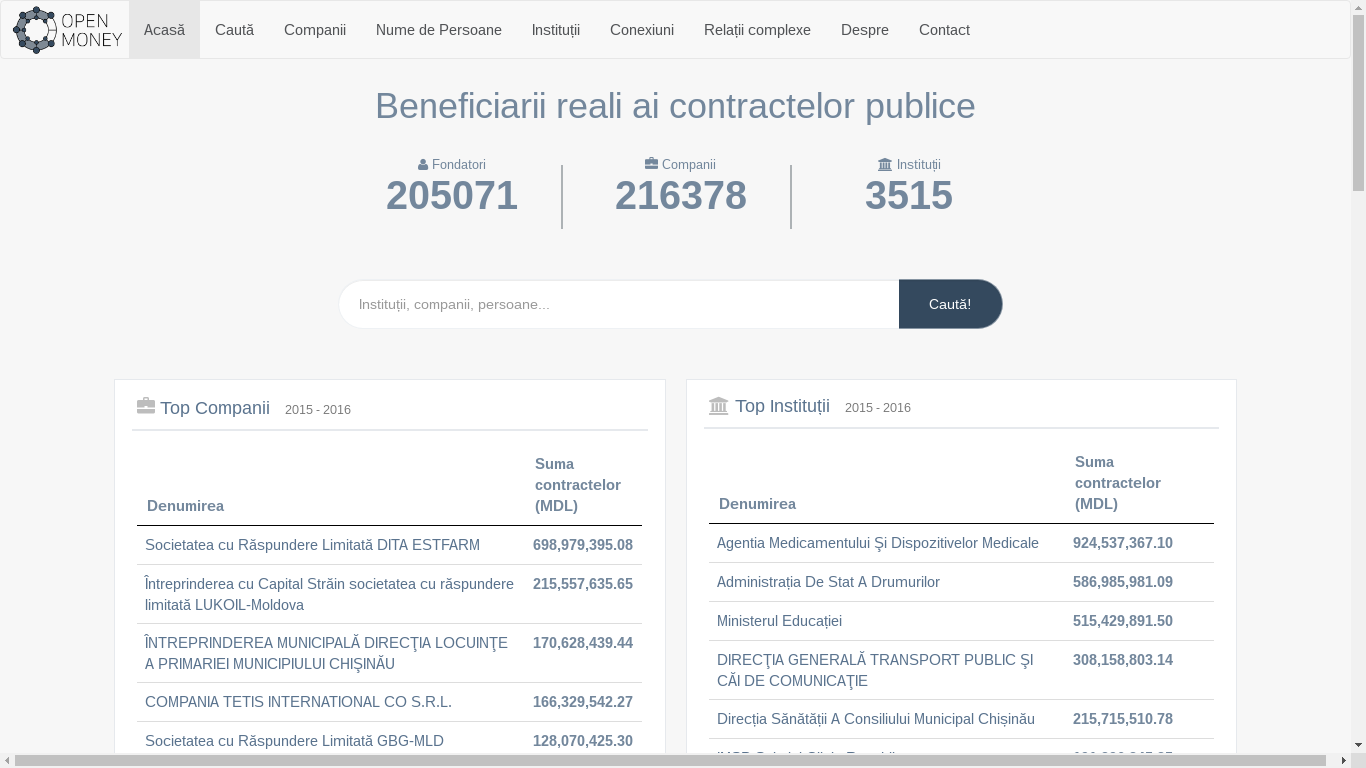
\includegraphics[width=17cm]{home.png} 
	\caption{ Home page }\label{fig4} 
	\end{figure}
	
\newpage
\subsection{Companies}
	\begin{figure}[!ht] 
	\renewcommand\thefigure{2} % Make this Figure I.3 
	\centering 
	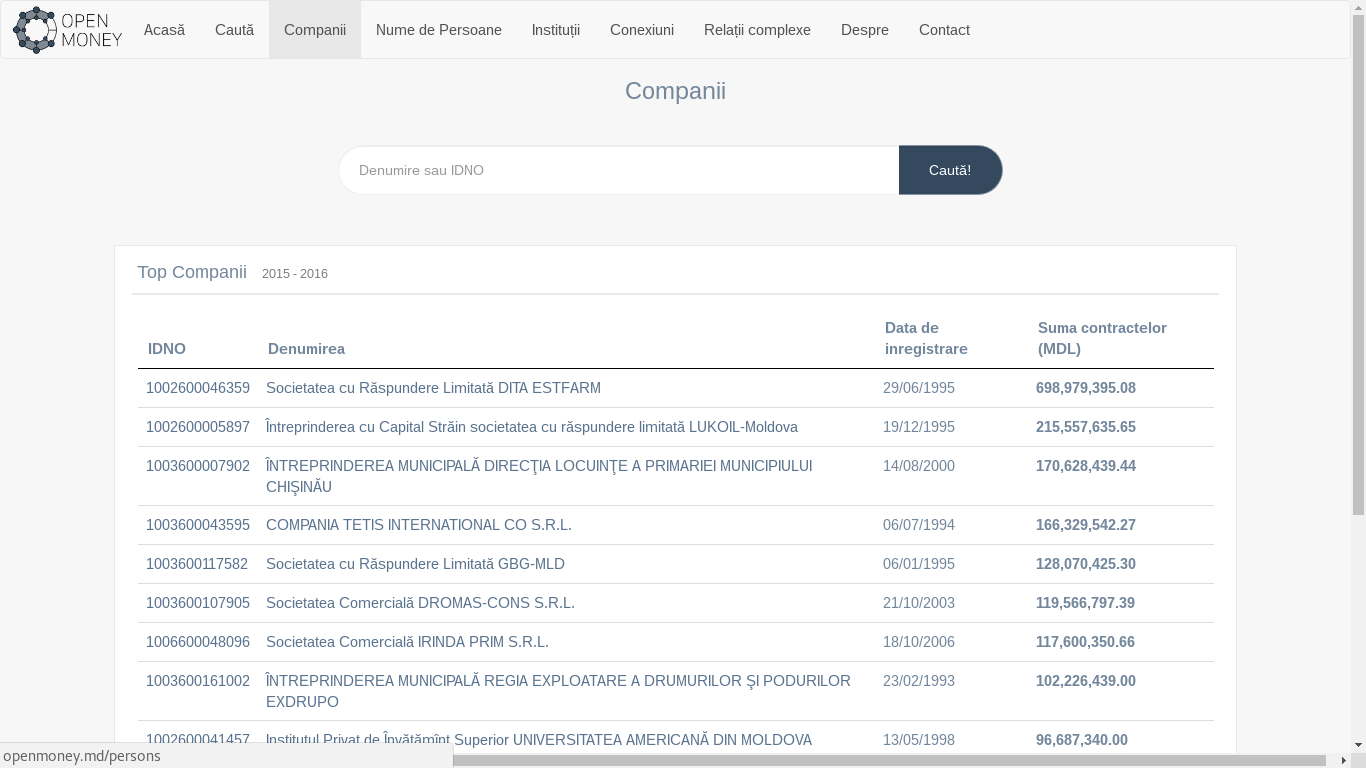
\includegraphics[width=17cm]{companies.png} 
	\caption{ Companies }\label{fig4} 
	\end{figure}
	
	\begin{figure}[!ht] 
	\renewcommand\thefigure{3} % Make this Figure I.3 
	\centering 
	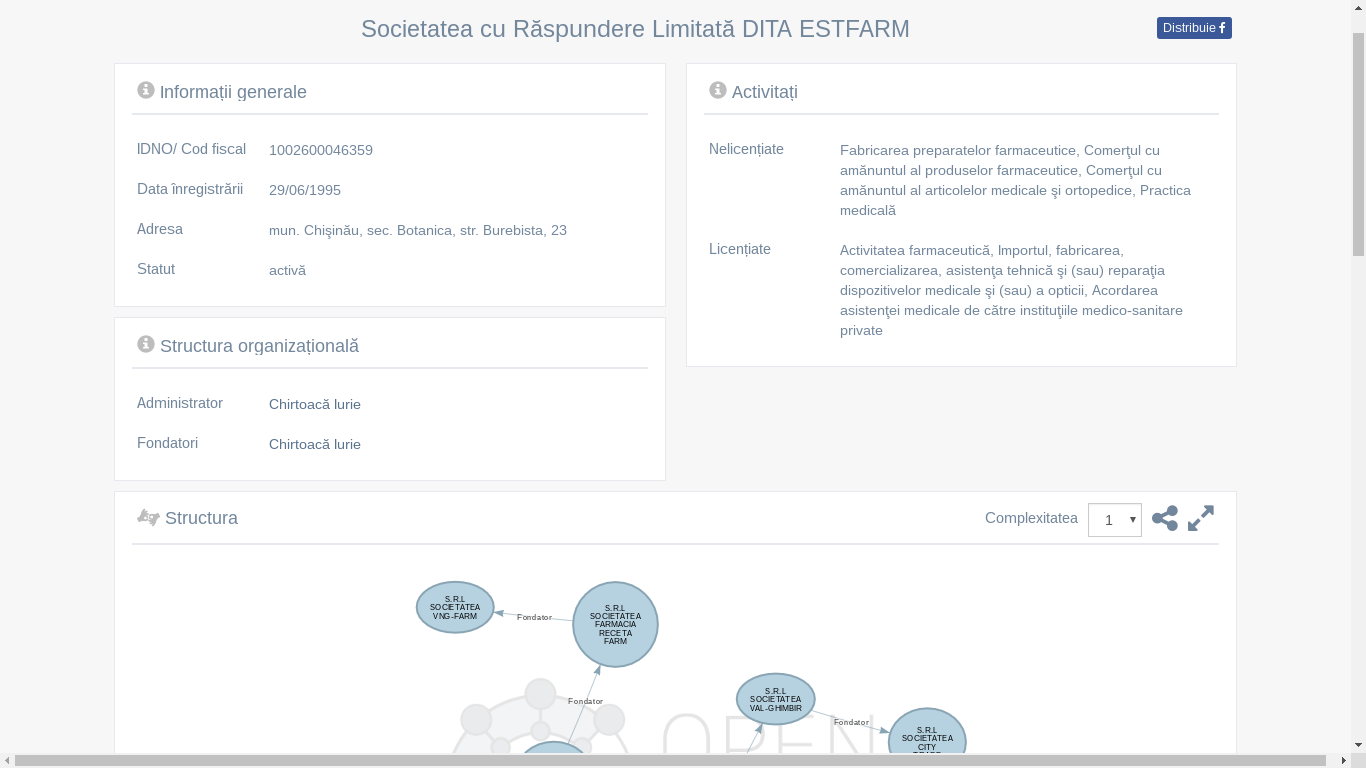
\includegraphics[width=17cm]{company_info.png} 
	\caption{ Company's information }\label{fig4} 
	\end{figure}
	
	\begin{figure}[!ht] 
	\renewcommand\thefigure{4} % Make this Figure I.3 
	\centering 
	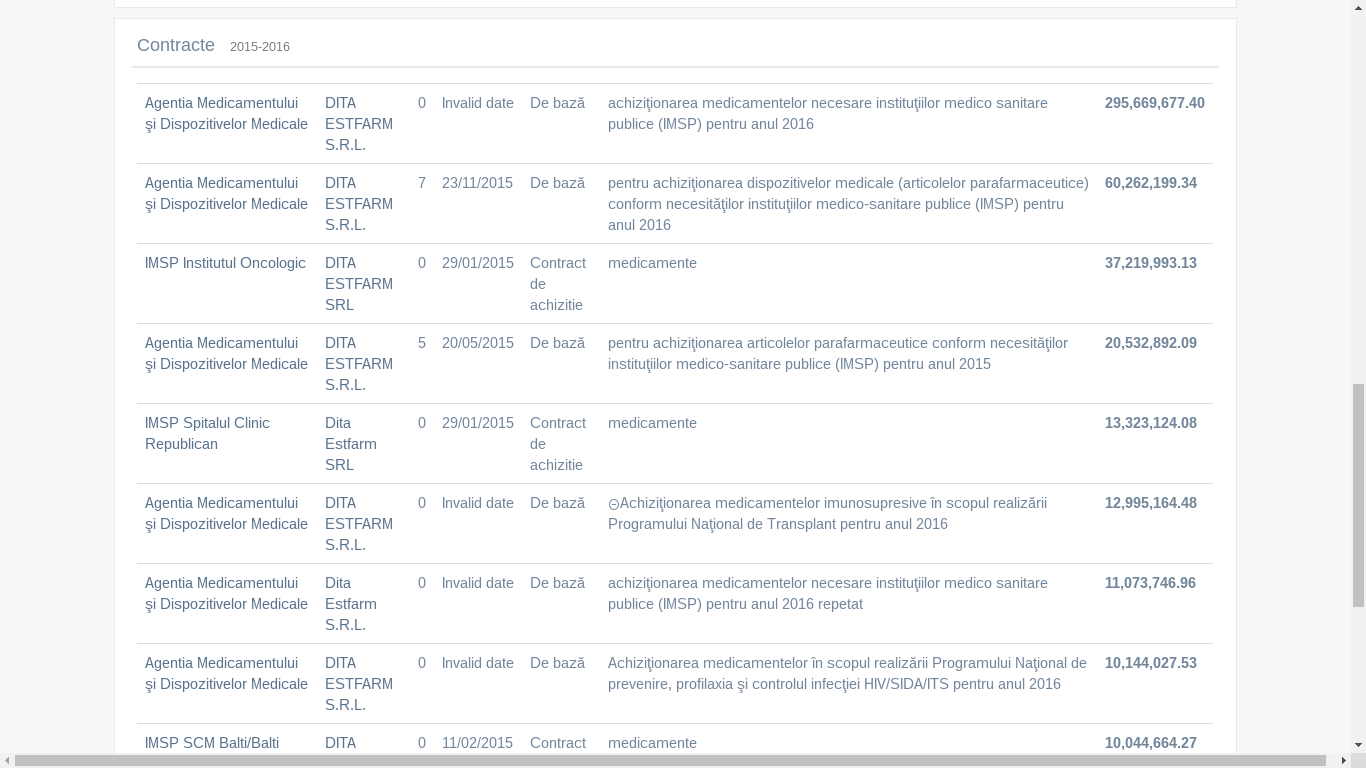
\includegraphics[width=17cm]{company_tenders.png} 
	\caption{ Company's tenders }\label{fig4}
	\end{figure}
	
\newpage
\subsection{Persons - }
	\begin{figure}[!ht] 
	\renewcommand\thefigure{5} % Make this Figure I.3 
	\centering 
	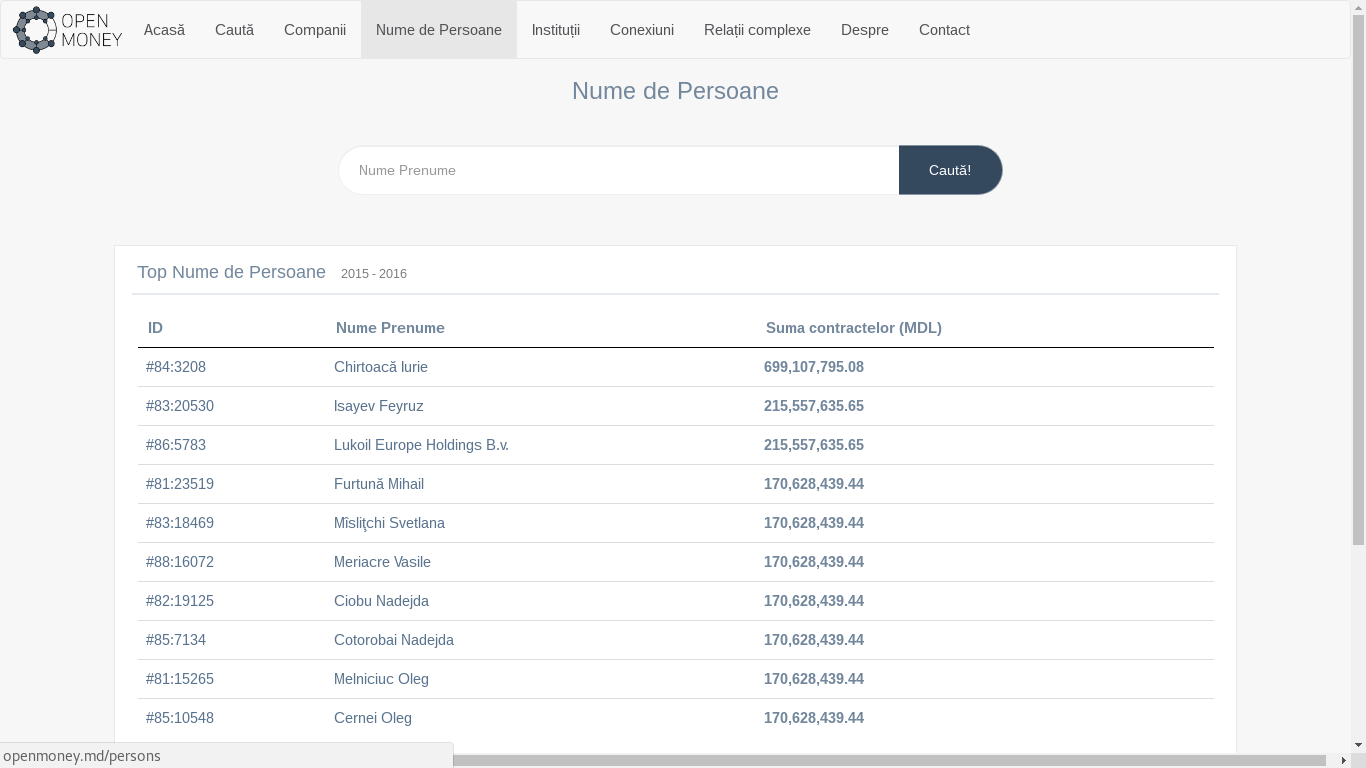
\includegraphics[width=17cm]{persons.png} 
	\caption{ Persons }\label{fig4} 
	\end{figure}
	
	\begin{figure}[!ht] 
	\renewcommand\thefigure{6} % Make this Figure I.3 
	\centering 
	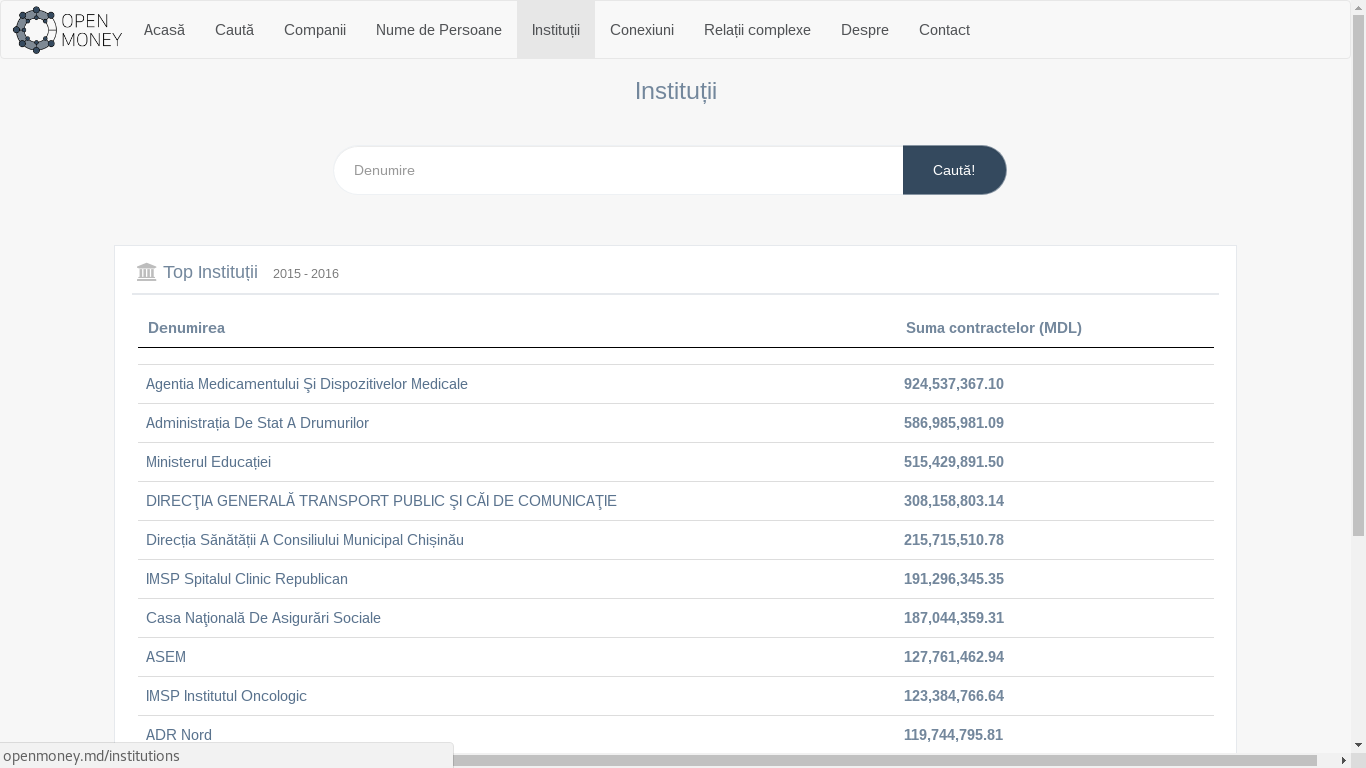
\includegraphics[width=17cm]{institutions.png} 
	\caption{ Institutions }\label{fig4} 
	\end{figure}
	
	\newpage
	\begin{figure}[!ht] 
	\renewcommand\thefigure{7} % Make this Figure I.3 
	\centering 
	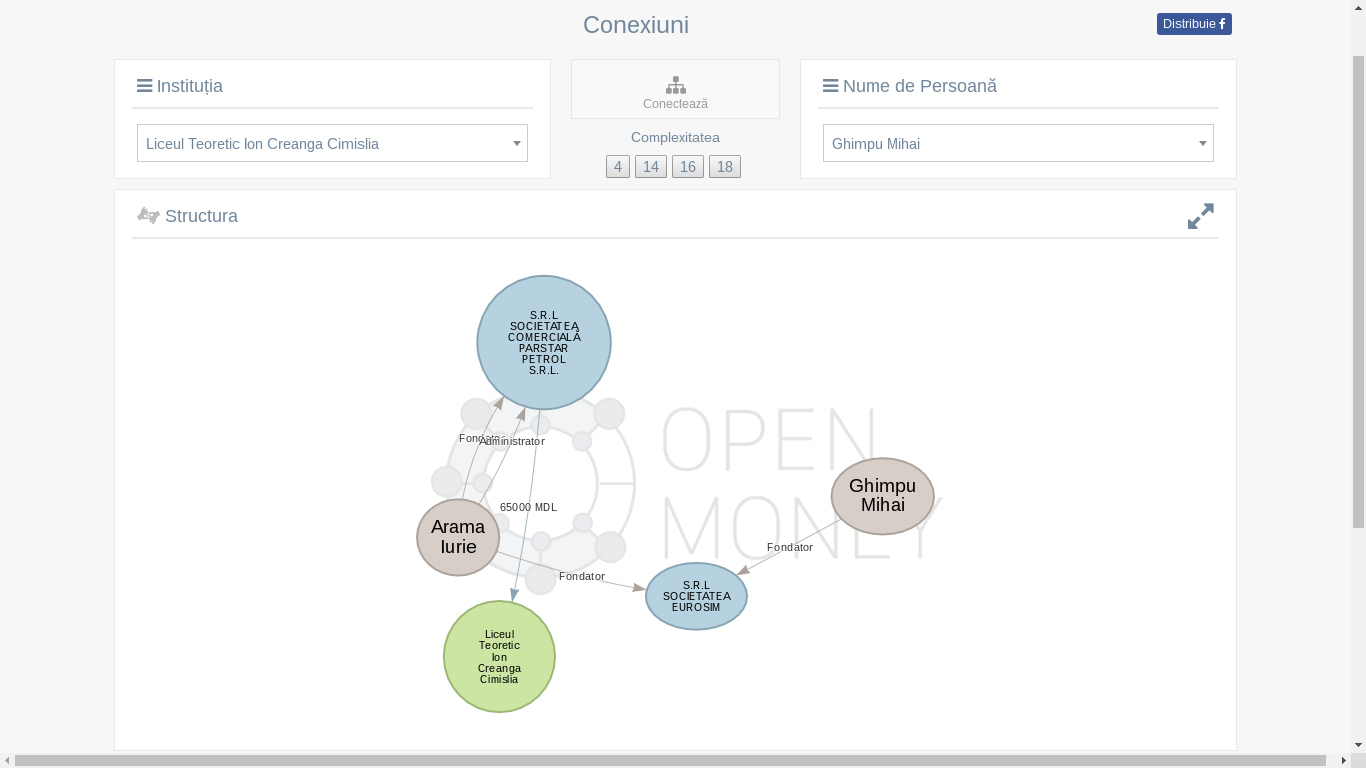
\includegraphics[width=17cm]{connections.png} 
	\caption{ Connections between a person and institution through UNDIRECTED relations (possible money flow) }\label{fig4} 
	\end{figure}
	
	\begin{figure}[!ht] 
	\renewcommand\thefigure{8} % Make this Figure I.3 
	\centering 
	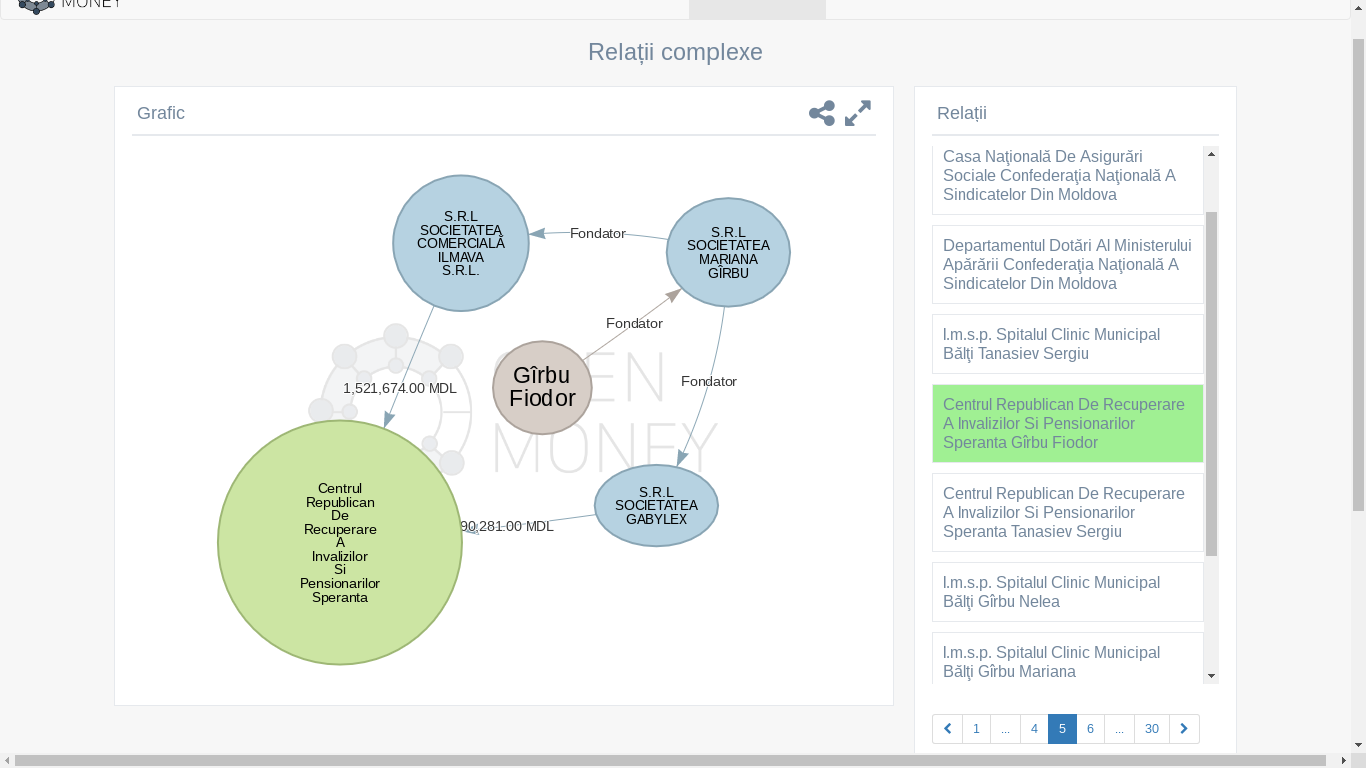
\includegraphics[width=17cm]{complex_relation.png} 
	\caption{ Complex relation - automatic detection of relation between person and institution where more companies that won tenders at the same institution are owned by same person in top level hierarchy only through DIRECTED relations }\label{fig4} 
	\end{figure}
	
	
	\newpage
	\begin{figure}[!ht] 
	\renewcommand\thefigure{9} % Make this Figure I.3 
	\centering 
	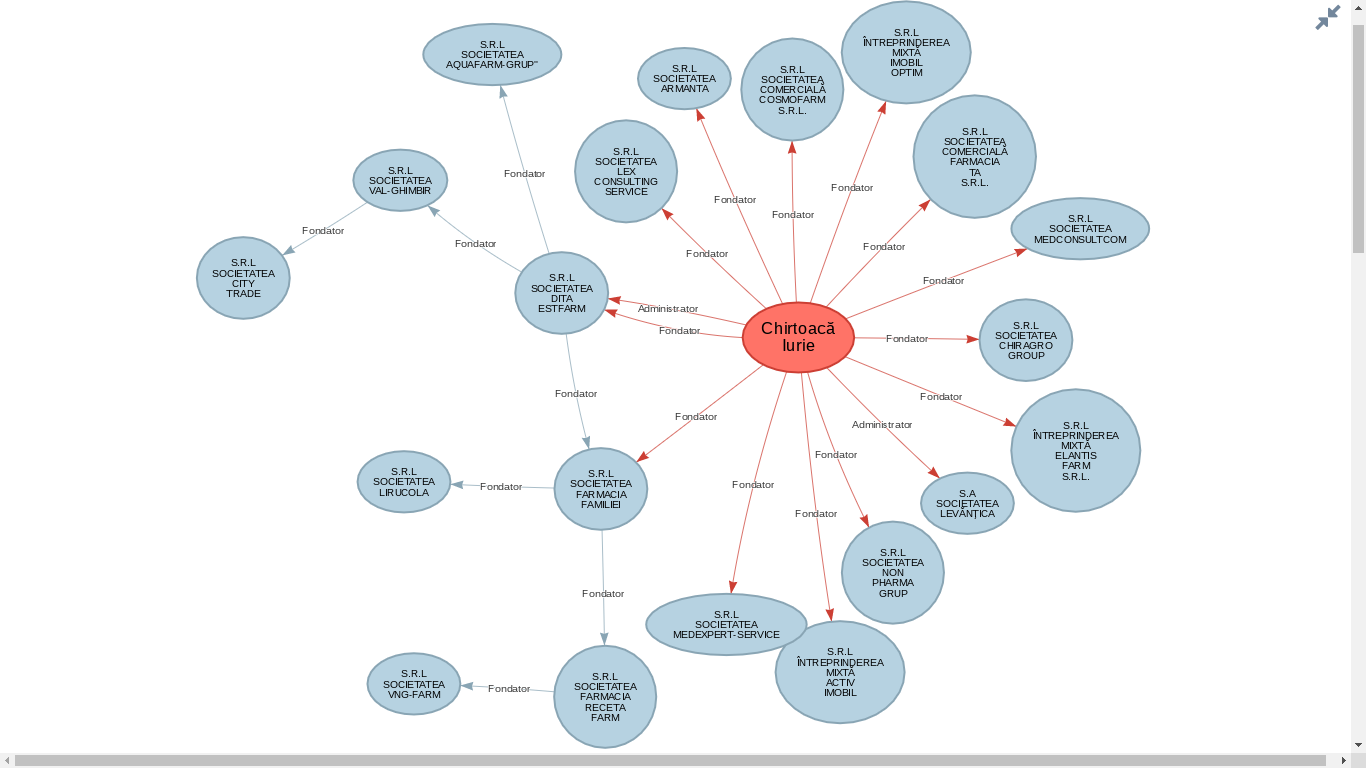
\includegraphics[width=17cm]{graph.png} 
	\caption{ General overview of hierarchy of foundation and ownership starting from an entity (person in that case) }\label{fig4} 
	\end{figure}

\newpage
\section{System realization}

\subsection{Used technologies}
It consists 2 parts: Backend for processing, and Frontend visualizing results for end user

BACKEND:
used technologies:
\begin{enumerate}
\item Java - as main language
\item Spring DI framework for wiring and in general for management of application components
\item Spring MVC framework as web layer for request handling
\item OrientDB - nosql graph database
\item Intellij IDEA - IDE for java development from Jetbrains team
\end{enumerate}

FRONTEND:
used technologies:
\begin{enumerate}
\item Javascript - as main language
\item Aurelia - javascript framework for browser application
\item Webstorm - IDE for javascript development from Jetbrains team
\end{enumerate}

\newpage
\subsubsection{JAVA}
	Java is a general-purpose computer programming language that is concurrent, class-based, object-oriented and specifically designed to have as few implementation dependencies as possible. It is intended to let application developers 'write once, run anywhere', meaning that compiled Java code can run on all platforms that support Java without the need for recompilation. Java applications are typically compiled to bytecode that can run on any Java virtual machine (JVM) regardless of computer architecture. As of 2016, Java is one of the most popular programming languages in use,articularly for client-server web applications, with a reported 9 million developers.
	 The major characteristics of Java are:

    The created programs are portable in a network. The source program is compiled into what Java calls bytecode, which can be run anywhere in a network on a server or client that has a Java virtual machine. The Java virtual machine interprets the bytecode into code that will run on the real computer hardware. This means that individual computer platform differences such as instruction lengths can be recognized and accommodated locally just as the program is being executed. Platform-specific versions of the program are no longer needed.
    The code is robust, here meaning that, unlike programs written in C++ and perhaps some other languages, the Java objects can contain no references to data external to themselves or other known objects. This ensures that an instruction can not contain the address of data storage in another application or in the operating system itself, either of which would cause the program and perhaps the operating system itself to terminate or "crash." The Java virtual machine makes a number of checks on each object to ensure integrity.
    Java is object-oriented, which means that, among other characteristics, an object can take advantage of being part of a class of objects and inherit code that is common to the class. Objects are thought of as "nouns" that a user might relate to rather than the traditional procedural "verbs." A method can be thought of as one of the object's capabilities or behaviors.
    In addition to being executed at the client rather than the server, a Java applet has other characteristics designed to make it run fast.
    Relative to C++, Java is easier to learn.
    Java was introduced by Sun Microsystems in 1995 and instantly created a new sense of the interactive possibilities of the Web. Both of the major Web browsers include a Java virtual machine. Almost all major operating system developers (IBM, Microsoft, and others) have added Java compilers as part of their product offerings.

	The Java virtual machine includes an optional just-in-time compiler that dynamically compiles bytecode into executable code as an alternative to interpreting one bytecode instruction at a time. In many cases, the dynamic JIT compilation is faster than the virtual machine interpretation.

	JavaScript should not be confused with Java. JavaScript, which originated at Netscape, is interpreted at a higher level, is easier to learn than Java, but lacks some of the portability of Java and the speed of bytecode. Because Java applets will run on almost any operating system without requiring recompilation and because Java has no operating system-unique extensions or variations, Java is generally regarded as the most strategic language in which to develop applications for the Web.

\newpage
\subsubsection{Spring DI}

Every Java-based application has a few objects that work together to present what the end-user sees as a working application. When writing a complex Java application, application classes should be as independent as possible of other Java classes to increase the possibility to reuse these classes and to test them independently of other classes while unit testing. Dependency Injection (or sometime called wiring) helps in gluing these classes together and at the same time keeping them independent.

\newpage
\subsubsection{Spring MVC}

The Spring Web MVC framework provides Model-View-Controller (MVC) architecture and ready components that can be used to develop flexible and loosely coupled web applications. The MVC pattern results in separating the different aspects of the application (input logic, business logic, and UI logic), while providing a loose coupling between these elements.

\newpage
\subsubsection{OrientDB}

OrientDB is an open source NoSQL database management system written in Java. It is a multi-model database, supporting graph, document, key/value, and object models, but the relationships are managed as in graph databases with direct connections between records. It supports schema-less, schema-full and schema-mixed modes. It has a strong security profiling system based on users and roles and supports querying with Gremlin along with SQL extended for graph traversal. OrientDB uses several indexing mechanisms based on B-tree and Extendible hashing, the last one is known as "hash index", there are plans to implement LSM-tree and Fractal tree index based indexes. Each record has Surrogate key which indicates position of record inside of Array list , links between records are stored either as single value of record's position stored inside of referrer or as B-tree of record positions (so-called record IDs or RIDs) which allows fast traversal (with O(1) complexity) of one-to-many relationships and fast addition/removal of new links. OrientDB is the second most popular graph database according to the DB-Engines graph database ranking.

\newpage
\subsubsection{Intellij IDEA }

IntelliJ IDEA  is a Java integrated development environment (IDE) for developing computer software. It is developed by JetBrains (formerly known as IntelliJ), and is available as an Apache 2 Licensed community edition, and in a proprietary commercial edition. Both can be used for commercial development.

\newpage
\subsubsection{Javascript }

JavaScript, often abbreviated as "JS", is a high-level, dynamic, untyped, and interpreted run-time language. It has been standardized in the ECMAScript language specification. Alongside HTML and CSS, JavaScript is one of the three core technologies of World Wide Web content production; the majority of websites employ it, and all modern Web browsers support it without the need for plug-ins. JavaScript is prototype-based with first-class functions, making it a multi-paradigm language, supporting object-oriented, imperative, and functional programming styles. It has an API for working with text, arrays, dates and regular expressions, but does not include any I/O, such as networking, storage, or graphics facilities, relying for these upon the host environment in which it is embedded.


\newpage
\section{Economic Evaluation of the Project}

Development is based on money obtained from grant. After finishing first version need to analize the possible additional features and to try to search for other investments in dependence of wanted features.

\subsection{SWOT analysis}

Strengths:
\begin{enumerate}
\item local support
\end{enumerate}

Weaknesses:
\begin{enumerate}
\item bad structure of egov open data
\end{enumerate}

Opportunities:
\begin{enumerate}
\item lack of similar products on the market
\end{enumerate}

Threats:
\begin{enumerate}
\item error on relation connections because of bad  structure of open data
\end{enumerate}


\newpage
\section*{Conclusion}
    This is very actual topic for our corrupt country, so even if it is naive to catch a real situation of corruption with such application i just try to do my best using my IT skills.
\end{document}
